\documentclass{ifacconf}

\usepackage{xcolor}
\usepackage{enumerate}
\usepackage{amsmath, amssymb,mathrsfs}
\usepackage{natbib}            % you should have natbib.sty
\usepackage{graphicx}          % Include this line if your 
                               % document contains figures,
%\usepackage[dvips]{epsfig}    % or this line, depending on which
                               % you prefer.

\usepackage{tikz,environ}
\usetikzlibrary{arrows,positioning,patterns,decorations.pathreplacing}

\tikzset{
    at xy split/.style 2 args={
        at={(#1,#2)}
    },
    a/.style={circle, draw=red},`'
    b/.style={rectangle, draw=blue}
}

\makeatletter
\newsavebox{\measure@tikzpicture}
\NewEnviron{scaletikzpicturetowidth}[1]{%
  \def\tikz@width{#1}%
  \def\tikzscale{1}\begin{lrbox}{\measure@tikzpicture}%
  \BODY
  \end{lrbox}%
  \pgfmathparse{#1/\wd\measure@tikzpicture}%
  \edef\tikzscale{\pgfmathresult}%
  \BODY
}
\makeatother

\def\bpf{\textnormal{\textit{Proof:}\hspace{1ex}}}
\def\epf{\hfill \mbox{\qed}}%$\Box$}

% predefined environments
%\begin{thm} ... \end{thm}		% Theorem
%\begin{lem} ... \end{lem}		% Lemma
%\begin{claim} ... \end{claim}	% Claim
%\begin{conj} ... \end{conj}	% Conjecture
%\begin{cor} ... \end{cor}		% Corollary
%\begin{fact} ... \end{fact}	% Fact
%\begin{hypo} ... \end{hypo}	% Hypothesis
%\begin{prop} ... \end{prop}	% Proposition
%\begin{crit} ... \end{crit}	% Criterion
%\begin{rem} ... \end{rem}    % Remark
%\begin{pf} ... \end{pf}      % Proof
%\begin{ack} ... end{ack}     % Acknowledgement

\providecommand{\abs}[1]{\left|#1\right|}
\providecommand{\norm}[1]{\left\|#1\right\|}
\newcommand{\blue}{\textcolor{blue}}
\newcommand{\green}[1]{\textcolor[rgb]{0,.5,0}{#1}}
\newcommand{\red}{\textcolor{red}}

\providecommand{\conv}{\text{conv}}
\providecommand{\vol}{\text{vol}}
\providecommand{\spann}{\text{span}}
\newcommand{\Obs}{\mathcal{O}}
\providecommand{\B}{\mathcal B}
\providecommand{\C}{\mathscr C}
\providecommand{\Xinfty}{{\mathscr X}^\infty}
\providecommand{\E}{\mathcal E}
\providecommand{\F}{\mathscr F}
\providecommand{\W}{\mathcal W}
\providecommand{\V}{\mathcal V}
\providecommand{\X}{\mathcal X}
\providecommand{\Y}{\mathcal Y}
\providecommand{\Z}{\mathcal Z}
\providecommand{\U}{\mathcal U}
\providecommand{\R}{\mathcal R}
\providecommand{\T}{\mathcal T}
\providecommand{\D}{\mathscr D}
\providecommand{\PP}{\mathbb P}
\providecommand{\RR}{\mathbb R}
\providecommand{\bfa}[1]{\mathbf{#1}}

\newcommand*{\Resize}[1]{\resizebox{\columnwidth}{!}{$#1$}}

\allowdisplaybreaks[4]

\begin{document}

\begin{frontmatter}

\title{Maximising the guaranteed feasible set for uncertain MPC schemes with chance constraints}%\thanksref{footnoteinfo}} 
% Title, preferably not more than 10 words.


\author{Rainer M. Schaich} 
\qquad\qquad\author{Mark Cannon}


\address{\mbox{Department of Engineering Science, University of Oxford, OX1 3PJ, UK} e-mail: \{rainer.schaich,mark.cannon\}@eng.ox.ac.uk}


          
\begin{keyword}                           % Five to ten keywords,  
Keyword 1; keyword 2;
\end{keyword}                             % keyword list or with the 
                                          % help of the Automatica 
                                          % keyword wizard


\begin{abstract}                          % Abstract of not more than 250 words.
This paper proposes a method of approximating positively invariant sets and $n$-step controllable sets of uncertain linear systems that are subject to chance constraints. The computed sets are robustly invariant and are guaranteed to satisfy the probabilistic constraints of the control problem. In contrast, existing methods based on random sampling are only able to satisfy such constraints with a fixed level of confidence. The proposed approach uses explicitly parametrised auxiliary disturbance sets, which are optimised subject to a constraint on their probability measure so as to maximise the relevant positively invariant or $n$-step controllable set. The results are illustrated by numerical examples.
\end{abstract}

\end{frontmatter}


\section{Introduction}
%
%
Positively invariant sets for uncertain linear systems have been researched for several decades, see e.g.~\cite{Kolmanovsky:1995,Kolmanovsky:1998,blanchini:2007}.
%
The properties of such sets and the algorithms to compute them are well known and documented in the literature.
%
As well as being objects of interest in their own right,
%In addition to pure analysis purposes, 
these sets are often used as terminal constraint sets in Model Predictive Control (MPC) in order to guarantee the feasibility of the control scheme at all times \citep[see e.g.][]{Mayne2014}.
%

For the methods presented in~\cite{Kolmanovsky:1998} and~\cite{blanchini:2007} to be applicable, the modelled uncertainty has to be constrained to a known disturbance set, in particular a convex polytopic or ellipsoidal set.
%
If constraints on the system do not have to be satisfied for all uncertainty realisations but instead are invoked for an arbitrary subset of the uncertainty set of sufficient size (or probability measure), then the problem becomes a chance constrained problem \cite[see e.g.][]{Kall1994}.
%
Control formulations of this kind can be addressed using a range of techniques including scenario optimization \citep[e.g.][]{Calafiore2010}, and sampling-based methods, \citep[e.g.][]{Margellos2014,Zhang2015,Fleming2016}.
%

Positively invariant sets based on samples of uncertain model parameters are often computationally expensive to determine and guarantees can only be given in a stochastic sense, namely with a certain confidence level.
%
The method presented in~\cite{Zhang2015} determines a set in which the probabilistic requirements are met with a given confidence and uses that set for subsequent analysis.
%
However, for simple probability distributions such as the uniform distribution considered in this paper, this approach does not require sampling; instead we can explicitly parametrise an auxiliary disturbance set in which all probabilistic conditions are met.
%
Using such a parametrised set, we can perform an optimisation
%the size of the positively invariant set 
%for the particular set 
in order to compute the largest positively invariant set while guaranteeing satisfaction of the probabilistic constraints, hence approximating the maximal positively invariant set for a chance-constrained problem.
%
Unlike sample based approaches, this method ensures probabilistic constraint satisfaction with certainty (rather than with a confidence level less than $1$, which is the case for sample-based methods).
%
A similar principle of using parametrised sets of a specified probability measure is used in $p$-efficiency theory~\citep{Dentcheva2009}, where the distribution is not required to be simple but the structure of the chance constraints is restrictive.

In order to formulate a robust MPC law for a chance constrained stochastic system while introducing a minimal amount of conservatism, we consider a closed-loop min-max formulation~\citep{Lee:1997}. This requires the determination of additional constraints.
%
The $n$-step controllable set for a given horizon $n$ and target set \citep[see e.g.][]{bertsekas71} has the property that, for every state in the $n$-step controllable set, there exists an admissible input sequence such that the system state enters the target set after $n$ steps, for any admissible sequence of uncertainty realisations.
%
Using a parametrised uncertainty set with specified probabilistic properties, chance constraints can be replaced by computationally convenient set operations that guarantee the satisfaction of the original chance constraints.
%
By maximising the size of the $n$-step controllable set we indirectly approximate the $n$-step controllable set of the probabilistically constrained system.

%The remainder of this paper elaborates the method in the following way:
%
This paper is organised  as follows:
In section~\ref{sec:setup} we present the problem formulation and derive, in section~\ref{ssec:approximating:MRPI}, conditions that define the positively invariant set under chance constraints. The corresponding conditions for the $n$-step controllable set are derived in section~\ref{ssec:approximating:n:step} and these are used to define an MPC law in section~\ref{ssec:mpc}.
%
The parametrisation of a parallelotope is discussed in~\ref{sec:volume:of:hypercube} and the general problem formulations introduced in section~\ref{sec:setup} are made precise for this parametrisation.
%
Two numerical examples are presented in section~\ref{sec:examples} to illustrate the proposed scheme in two dimensions and in section~\ref{sec:conclusion} we conclude the presentation and sketch possible extensions to the presented scheme.

\textit{Notation.} Given sets $A,B\subset\RR^d$, $A\oplus B = \{x:x=a+b,\, a\in A,\, b\in B\}$ denotes the Minkowski sum and $A\ominus B = \{x: x+b \in A \ \forall b\in B\}$ the Pontryagin difference. We denote the image and pre-image of $C\subset\RR^d$ under the linear map $A:\RR^d\rightarrow\RR^d$ respectively as $AC = \{y\in\RR^d:Ax=y,\, x\in C\}$ and $A^{-1}C = \{y\in\RR^d:Ay\in C\}$. The $d$-dimensional volume of $C\subset\RR^d$ is denoted by $\vol(C)$. 
%
We define $v$ as a random parameter on a probability space $(\V,\F,\PP)$ and denote the probability of an event $E(v)$ as $\PP\{v\in\V : E(v)\}$.
%; throughout this paper the probability density of $v$ is assumed to be uniform.
%
For a positive definite matrix $P$ we write $\|x\|_P^2 = x^TPx$, and the set $\B_P(r) = \{x\in\RR^d:x^TPx\leq r^2\}$ denotes the $P$-ball of radius $r$ centred at the origin. The constraint $\Gamma x\leq \bfa{1}$, where $\Gamma\in\RR^{m\times n}$ and $\bfa{1}$ is a vector of ones in $\RR^m$, is understood to apply element-wise.


\section{Problem formulation}\label{sec:setup}
%


The discrete time system we consider is given by
%
\begin{equation}\label{eq:system}
	x^+ = Ax + Bu + w ,
\end{equation}
%
where the state $x$ and control input $u$ are subject to constraints defined in terms of compact, convex polytopic sets $\X$, $\U$:
\begin{equation}\label{eq:state_input:constraints}
\begin{aligned}
&x \in\X = \bigl\{x\in\RR^d : E_ix\leq 1, \, i\leq M_\X\bigr\}, \\
&u\in\U = \bigl\{u\in\RR^{q_\U} : F_i u\leq 1, \, i\leq M_\U\bigr\},
\end{aligned}
\end{equation} 
and the disturbance input $w$ is subject to the constraint
\begin{equation}\label{eq:disturbance}
w\in\W = \bigl\{w\in\RR^{q_\W}:G_i w\leq 1,\, i\leq M_\W \bigr\}.
\end{equation}
%
We furthermore consider the output variable $y$,
%
\[%\begin{equation}\label{eq:output}
	y = Cx + Du + v
\]%\end{equation}
%
which depends on the random variable $v$,
\[
v\in\V = \bigl\{v\in\RR^{q_\Y}:\Gamma_i v\leq 1, \ i\in M_\V\bigr\}. 
\]
Throughout this paper $v$ is assumed to be uniformly distributed on $\V$.
%Throughout this paper the probability density function of $v$ is assumed to be uniform.
%
The output variable $y$ is subject to the chance (or probabilistic) constraint
%
\begin{equation}\label{eq:probabilistic:constraint}
	\PP\bigl\{ v \in \mathcal{V} : y = Cx + Du + v \in \mathcal{Y} \bigr\}\geq p
\end{equation}
%
for given $p\in(0,1]$, with
\[
\Y=\bigl\{y\in\RR^{q_\Y} : H_i y\leq h_i, \ i\leq M_\Y\bigr\}.
\]

We make  use of the following proposition.
%

\vspace{0.5\baselineskip}
\begin{prop}\label{prop1}
Let $v\in\V$ be a uniformly distributed random variable and let $\V^\prime\subseteq\V$ be such that $\vol(\V^\prime)\geq p$, then every $q\in\Z\ominus\V^\prime$ satisfies $\PP\{v\in\V : q+v\in\Z\}\geq p$.
\end{prop}
%

\bpf
%
For any given $q\in\Z\ominus\V^\prime$, the definition of the Pontryagin difference implies that
\[
q+v\in\Z \quad \text{whenever} \quad  v\in\V^\prime.
\]
Therefore, for every $q\in\Z\ominus\V^\prime$, the probability of the event that $q+v$ lies in $\Z$ can be no less than the probability of the event that $v$ lies in $\V^\prime$. It follows that 
\[
\PP\{ v\in\V : q + v\in \Z\} \geq \PP\{\V^\prime\} = \vol(\V^\prime)
\]
and hence $\PP\{ v\in\V : q + v\in \Z\} \geq p$ if $\V^\prime$ is such that $\vol(\V^\prime) \geq p$.
% Using the fact that $\PP\{\{q\}\oplus\V^\prime\subseteq\Z\} = \PP\{\V^\prime\} = \vol(\V^\prime)$ for all $q\in\Z\ominus\V^\prime$ we have
% %
% \begin{align*}
% &\PP\{v\in\V : q+v\in\Z\} 
% =\PP\{v\in \V^\prime\cup(\V\setminus\V^\prime) : q + v \in \Z, \ ()\subseteq\Z\} \\
% &=\PP\{\{q\}\oplus\V^\prime\subseteq\Z\} + \PP\{\{q\}\oplus(\V\setminus\V^\prime)\subseteq\Z\} \\
% &\geq\PP\{\{q\}\oplus\V^\prime\subseteq\Z\}\\ &=\vol(\V^\prime)\geq p. 
% \end{align*}
%\mbox{}\vspace{-0.5\baselineskip}
\epf
%

Note that for polytopic $\Z$ and $\V^\prime$ the set $\Z\ominus\V^\prime$ can be computed explicitly and is itself polytopic.

In the remainder of this paper we discuss how~$\V^\prime$ can be chosen in order to obtain the largest guaranteed $n$-step controllable set for a given target set and the largest guaranteed positively invariant set for the system (\ref{eq:system}) subject to the robust constraints~(\ref{eq:state_input:constraints}) and the chance constraint (\ref{eq:probabilistic:constraint}).


\section{Approximating the guaranteed invariant set}\label{ssec:approximating:MRPI}
%
First we discuss how to extend existing methods to calculate the maximal robust positively invariant (MRPI) set (see e.g.~\cite{blanchini:2007}) in such a way that all states in the MRPI set produce only feasible successor states for a given feedback controller $u = Kx$.
%
Thus we seek to determine a set of initial conditions for which all possible trajectories of (\ref{eq:system}) subject to (\ref{eq:disturbance}) satisfy the robust constraints~(\ref{eq:state_input:constraints}) and probabilistic constraint (\ref{eq:probabilistic:constraint}). Denoting the largest such set as $\Xinfty$ we have
\begin{multline*}
\Xinfty = \Bigl\{x_0\in\X: \\
\begin{aligned}
% &x_k = (A+BK)^k x + \sum_{i=1}^{k} (A+BK)^{k-i} w_{k-i}\\
% &x_{k+1} = (A+BK)^{k+1} x + \sum_{i=1}^{k+1} (A+BK)^{k+1-i} w_{k+1-i}\\
&x_{k+1} = (A+BK)^{k+1} x_0 + \sum_{i=0}^{k} (A+BK)^{k-i} w_{i}\\
&x_{k+1}\in\X\\
&Kx_k\in\U\\
&\PP\{v\in\V : (C+DK)x_k+v\in\Y\}\geq p 
\end{aligned}\\
\forall w_k\in\W,\, \forall k\geq 0 \Bigr\} .
\end{multline*}
%
% \begin{multline}\label{eq:alternative:MRPI:set}
% 	X^\infty = \Bigl\{x\in\X: \\
% \begin{aligned}&x_k = (A+BK)^k x + \sum_{i=1}^{k} (A+BK)^{k-i-1} w_{k-i}\\
% 	&x_k\in\X\\
% 	&(C+DK)x_k+v\in\Y\\
% 	&\forall w_j\in\W,\ \forall v\in \V^\prime,\ \forall k\geq 0 \Bigr\}
% \end{aligned} 
% \end{multline}
%
% It is obvious that $X^\infty$ contained in the invariant set of the original problem~$\Xinfty$:
For a given set $\V^\prime$, let $X^\infty$ denote the set
%
\begin{multline}\label{eq:alternative:MRPI:set}
	X^\infty = \Bigl\{x_0\in\X: \\
\begin{aligned} 
%&x_k = (A+BK)^k x + \sum_{i=1}^{k} (A+BK)^{k-i} w_{k-i} \\
&x_{k+1} = (A+BK)^{k+1} x_0 + \sum_{i=0}^{k} (A+BK)^{k-i} w_{i} \\
&x_{k+1}\in\X \\ 
&Kx_k\in\U \\
&(C+DK)x_k+v_k\in\Y
\end{aligned}\\
\forall w_k\in\W,\ \forall v_k\in \V^\prime,\ \forall k\geq 0 \Bigr\} .
\end{multline}
% \begin{equation}
% 	\Xinfty = \left\{x\in\X: \begin{aligned}&x_k = (A+BK)^k x + \sum_{i=1}^{k} (A+BK)^{k-i-1} w_{k-i}\\
% 	&x_k\in\X\\
% 	&\PP\{(C+DK)x_k+v\in\Y\}\geq p\\
% 	&\forall w_j\in\W,k\geq 0\end{aligned} \right\}
% \end{equation}
%
Then from Proposition~\ref{prop1}, the inclusion $X^\infty\subseteq\Xinfty$ necessarily holds for any $\V^\prime\subseteq\V$ with probability measure $\PP\{\V^\prime\} \geq p$. Furthermore, by maximising the volume of $X^\infty$, we can improve the approximation of $\Xinfty$.


In order to determine an algorithm to compute $X^\infty$ we rewrite the conditions in~\eqref{eq:alternative:MRPI:set} by introducing the set of all possible successor states~$\D_k(X)$ of states in $X$ after $k$ time steps:
%
\begin{align*}
	\D_k(X) &= (A+BK)^{k}X\oplus\W\oplus\dots\oplus(A+BK)^{k-1}\W\\
	&= (A+BK)^k X\oplus \bigoplus_{i=0}^{k-1}(A+BK)^i\W
\end{align*}
%
Defining $\R = (C+DK)^{-1}(\Y\ominus\V^\prime)$ we can abbreviate the conditions defining $X^\infty$ in~\eqref{eq:alternative:MRPI:set} to
%
\begin{equation}\label{eq:containment:condition:alternative:MRPI}
\D_k(X^\infty)\subseteq\X\cap\R
\end{equation}
%
for all $k\geq0$.
%
Using these conditions we can express $X^\infty$ directly as
%
\begin{gather}
X^\infty = %\bigcap_{k\geq0}(A+BK)^{-k}\Bigl((\X\cap\R)\ominus\bigoplus_{i=0}^{k-1}(A+BK)^i\W\Bigr) \\
\bigcap_{k\geq0} \E_k, \\
\E_k = (A+BK)^{-k}\biggl[(\X\cap\R)\ominus\bigoplus_{i=0}^{k-1}(A+BK)^i\W\biggr] . \label{eq:Ek:subtract}
\end{gather}
% \begin{equation}\label{eq:direct:formulation:MRPI:with:intersection}
% 	X^\infty = \bigcap_{k\geq0}\underbrace{(A+BK)^{-k}\left((\X\cap\R)\ominus\bigoplus_{i=0}^{k-1}(A+BK)^i\W\right)}_{\E_k}.
% \end{equation}
%
Due to its definition~$\E_k$ satisfies $\D_k(\E_k)\subseteq\X\cap\R$ for each $k\geq0$, furthermore it can be shown that $\E_k$ expands exponentially and therefore $X^\infty$ is finitely determined  (see Theorem~\ref{thm2} below).
%
In order to compute $X^\infty$ we define the sequence $X_0,X_1,\ldots$ via the iteration:
%
\begin{equation}\label{eq:MRPI:sequence}
\begin{aligned}
  & X_0 = \X \\
  & \begin{aligned}
      & Z_k = X_k\cap\R\\
      & X_{k+1} = Z_k\cap(A+BK)^{-1}(Z_k\ominus\W)
    \end{aligned} 
  \ \Biggr\} \ \ k = 1,2,\ldots
\end{aligned}
\end{equation}
%
%with $X_0= \X$.
Clearly $X_k = \bigcap_{l=0,\ldots,k}\E_l$ and, analogously to the conventional MRPI calculation~\citep{Kolmanovsky:1998}, the iteration therefore gives $X_k = X^\infty$ once $X_k\subseteq X_{k+1}$.

\vspace{0.5\baselineskip}
\begin{thm}\label{thm2}
Let $\Gamma$ be a matrix such that $\Gamma x\leq\bfa{1}$ and $-\Gamma x\leq\bfa{1}$ for all $x\in\X$ and let $\bigl((A+BK),\Gamma\bigr)$ be observable, then the iteration~\eqref{eq:MRPI:sequence} %terminates after a finite number, $N$, of iterations, such that 
yields $X_{k+1}=X_k$ for all $k\geq N$ and hence $X_k=X^\infty$ for some finite integer $N$.
\end{thm}
%
\bpf
%
The observability of the pair $\bigl((A+BK),\Gamma\bigr)$ implies that $X_{d-1}$ is compact, since 
\begin{align*}
X_{d-1} 
&\subseteq\bigcap_{k\leq d-1}(A+BK)^{-k}\X\\
&\subseteq \Bigl\{x:\pm\Gamma x\leq\bfa{1}\wedge\dots\wedge\pm\Gamma(A+BK)^{d-1} x\leq\bfa{1} \Bigr\}\\
& = \bigl\{x:\pm\Gamma \Obs x\leq \bfa{1}\bigr\}
\end{align*}
where $\Obs$ is the (full rank) observability matrix.

Let~$P$ be such that 
\[
(A+BK)^TP(A+BK) \leq \rho^2P
\]
holds, where $\rho$ denotes the spectral radius of $A+BK$.
%
To see that $\E_k$ grows exponentially let $\W\subseteq\B_P(r)$ then
%
\begin{multline*}
  \bigoplus_{i=0}^{k-1}(A+BK)^i\W \subseteq \bigoplus_{i=0}^{k-1}(A+BK)^i\B_P(r)\\
  \subseteq\bigoplus_{i=0}^{k-1}\B_P(\rho^i r) = \B_P\biggl(\sum_{i=0}^{k-1}\rho^i r\biggr)\subseteq\B_P\Bigl(\frac{r}{1-\rho}\Bigr) .
\end{multline*}
%
It follows that the subtrahend in square brackets on the RHS of (\ref{eq:Ek:subtract}) is bounded for all $k$ by $\B_P\bigl(r / (1-\rho)\bigr)$.
%It follows that the RHS of (\ref{eq:Ek:subtract}) consists of an expanding minuend and a bounded subtrahend.
%
Therefore 
%$\E_k$ expands exponentially. Hence 
the iteration (\ref{eq:MRPI:sequence}) must either yield $X_N = \emptyset$ for finite $N$
(in which case $X^\infty=\emptyset$) or,
since $X_{d-1}$ is bounded and $\E_k$ expands exponentially, there must exist a finite $N$ such that $X_{N}\cap\E_{N+1}=X_N$ and hence $X_N=X^\infty$.
%
\epf

An optimisation problem whose solution approximates the maximal guaranteed positively invariant set $\Xinfty$ can therefore be formulated as
%
\begin{subequations}\label{seq:optimisation:MRPI:abstract}
\begin{align}
		& \max_{\V^\prime} \vol(X^\infty) \\
%\end{align}
%
\intertext{subject to}
%
%\begin{align}
	& \V^\prime\subseteq\V \\
% \end{equation}
% %
% \begin{equation}
	& \vol(\V^\prime)\geq p\cdot\vol(\V)
\end{align}
\end{subequations}
%
In section~\ref{sec:volume:of:hypercube} we discuss how this optimisation can be solved using a parallelotope parameterisation of~$\V^\prime$.


\section{Approximating the guaranteed $n$-step controllable set}\label{ssec:approximating:n:step}
%
We now turn our attention to the $n$-step controllable set~$\C_n(\T)$ for a given target set~$\T$.
%
This is defined as the set of initial conditions $x_0\in\X$ such that a sequence of control inputs exists that drives the state in $n$ steps to the target set, so that $x_n\in\T$ for all admissible disturbance sequences 
$w_k\in\W$, $k=0,\ldots,n-1$, while guaranteeing that the robust state and input constraints 
%$x_k\in\X$, $u_k\in\U$
(\ref{eq:state_input:constraints}) and the probabilistic constraint~(\ref{eq:probabilistic:constraint}) are satisfied.
%
Thus $\C_n(\T)$ can be expressed as follows.
%
\begin{multline*}
\C_n(\T) = \Bigl\{x_0\in\X: \exists \bigl\{u_0(\cdot),\ldots,u_{n-1}(\cdot)\bigr\}\\
\begin{aligned}
&x_{k+1} = A^{k+1} x_0 + \sum_{i=0}^{k} A^{k-i}B u_{i}(x_{i}) + \sum_{i=0}^{k} A^{k-i} w_{i}\\
&x_n\in\T\\
&x_{k+1}\in\X\\
&u_k(x_k)\in\U\\
&\PP\bigl\{v\in\V : Cx_k + Du_k(x_k) +v \in\Y\bigr\}\geq p
\end{aligned}\\
\forall w_k\in\W,\, \forall k\in\{ 0, \ldots , n-1\} \Bigr\}	
\end{multline*}
% \begin{equation}
% 	\C_n(\T) = \left\{x\in\X:\begin{aligned}&x_k = (A+BK)^k x + \sum_{i=1}^{k} (A+BK)^{k-i-1} w_{k-i}\\
% 	&x_N\in\T\\
% 	&x_k\in\X\\
% 	&\PP\{(C+DK)x_k+v\in\Y\}\geq p\\
% 	&\forall w_j\in\W,k\geq 0\end{aligned} \right\}	
% \end{equation}
%
Using Proposition~\ref{prop1} it is easy to verify that the set $C_n(\T)$ defined by
%
\begin{multline*}
C_n(\T) = \Bigl\{ x_0\in\X: \exists \bigl\{u_0(\cdot),\ldots,u_{n-1}(\cdot)\bigr\}\\
\begin{aligned}
&x_{k+1} = A^{k+1} x_0 + \sum_{i=1}^{k} A^{k-i}B u_{i}(x_{i}) + \sum_{i=1}^{k} A^{k-i} w_{i}\\
&x_N\in\T\\
&x_{k+1}\in\X\\
&u_k(x_k)\in\U \\
&Cx_k+Du_k(x_k) + v_k \in\Y
\end{aligned}\\
\forall w_k\in\W,\, \forall v_k\in \V^\prime,\, \forall k\in\{0,\dots,n-1\} \Bigr\}	
\end{multline*}
% \begin{equation}
% 	C_n(\T) = \left\{x\in\X:\begin{aligned}&x_k = (A+BK)^k x + \sum_{i=1}^{k} (A+BK)^{k-i-1} w_{k-i}\\
% 	&x_N\in\T\\
% 	&x_k\in\X\\
% 	&(C+DK)x_k+v\in\Y\\
% 	&\forall w_j\in\W,v\in \V^\prime,k\in\{0,\dots,N\}\end{aligned} \right\}	
% \end{equation}
%
is necessarily contained in $\C_n(\T)$ for any $\V^\prime\subseteq\V$ with probability measure $\PP\{\V^\prime\} \geq p$.
%
As in the case of positively invariant sets, fixing $\V^\prime$ to be a polytopic set leads to a computationally tractable optimisation for the maximisation of~$C_n$. This suggests an algorithm for constructing $C_n$ as a polytopic approximation of~$\C_n$ by optimising~$\V^\prime$ so as to maximise the volume of~$C_n$.
% indirectly improves the approximation of $\C_n$.
%
It is known that 
%$C_n(\T) = C^n_1(\T) \doteq C_1(C_1(\cdots C_1(\T)\cdots))$ 
$C_n(\T) = C^n_1(\T) \doteq C_1 \circ C_1 \circ \cdots \circ C_1(\T)$ 
\citep[see e.g.][]{blanchini:2007}, which allows the use of simple computational geometry algorithms.

In particular, the one-step controllable set $C_1(\T)$ for the target set 
\[
\T = \Bigl\{x\in\RR^d : J_i x\leq1,\ i\leq M_\T\Bigr\}
\]
is given by the projection of
$L_1(\T)\subset \RR^{d+q_{\U}}$, 
%$L_1(\T)\subset \RR^d\times \RR^{q_{\U}}$, 
defined by
%
\begin{multline*}
L_1(\T) = \Bigl\{(x,u)\in (\X,\U): \\
\begin{aligned}
& Cx+Du + v\in\Y \\
& Ax+Bu+w\in\T
\end{aligned}\\
\forall v\in\V^\prime,\, \forall w\in\W\Bigr\} ,
%\end{aligned}
\end{multline*}
% \begin{equation}
% 	L_1(\T) = \left\{(x,u):\begin{aligned}
% 	x\in\X, u\in\U, Cx+Du + v\in\Y\;\forall v\in\V^\prime,\\
% 	Ax+Bu+w\in\T\;\forall w\in\W
% 	\end{aligned}\right\}
% \end{equation}
%
onto the $x$-subspace.
%
Thus
\[
C_1(\T) = \{ x : \exists u \ \text{such that} \ (x,u)\in L_1(\T)\}.
\]
As all involved sets are polytopic, $L_1(\T)$ is polytopic and its exact projection can be determined computationally.

A set $C_n(\T)$ approximating the $n$-step controllable set $\C_n(\T)$ is then given by the solution of the optimisation:
%
\begin{subequations}\label{seq:optimisation:n:step:set:abstract}
\begin{align}
	& \max_{\V^\prime} \vol(C_n(\T))
%\end{equation}
\intertext{subject to}
%\begin{align}
	& \V^\prime\subseteq\V  \\
% \end{equation}
% %
% \begin{equation}
	& \vol(\V^\prime)\geq p\cdot\vol(\V)
\end{align}
\end{subequations}
The property $C_n(\T)\subseteq \C_n(\T)$ then guarantees the existence of a control sequence such that the constraints~(\ref{eq:state_input:constraints}) and (\ref{eq:probabilistic:constraint}) are met and $x_n\in\T$ for all $x_0\in C_n(\T)$.

Note that an additional improvement to the $n$-step controllable set $C_n(\T)$ could be obtained by introducing $\V_1^\prime,\dots,\V_{n-1}^\prime$, to allow different sets $\V_i^\prime$ at each stage.
% introducing $(n-1)\times 2d$ additional decision variables.

\section{Model Predictive Control}\label{ssec:mpc}

The method proposed for computing $n$-step controllable sets in section~\ref{ssec:approximating:n:step} can be used to formulate a chance constrained Model Predictive Control law. In order to minimise conservatism while guaranteeing constraint satisfaction, a closed loop MPC scheme should be used \citep[see e.g.][]{Lee:1997}.
This involves computing (offline) the set $X^\infty$ using \mbox{(\ref{seq:optimisation:MRPI:abstract}a-c)}, and the 
sets $C_{i}(X^\infty) = C_1\bigl(C_{i-1}(X^\infty)\bigr)$ and $L_{i}(X^\infty) = L_1\bigl(C_{i-1}(X^\infty)\bigr)$ 
for $i=1,\ldots,n$ by repeated application of (\ref{seq:optimisation:n:step:set:abstract}a-c) with $C_0(X^\infty)= X^\infty$.
Online, at each time step $k=0,1,\ldots$, a min-max MPC law is defined by 
\[
u_k = u^{(n)}(x_k)
\]
where $u^{(n)}(x_k)$ is the solution of
%
\[%\begin{equation}
\begin{aligned}
\Bigl( u^{(n)} (x_k) , w^{(n)} (x_k,u) \Bigr) &= \arg \min_{u} \Bigl\{ \max_{w\in\W} J^{(n)}(x_k,u,w)  
\\
&\ \quad \text{subject to}\ (x_k, u) \in L_n(\T)
\Bigr\}
\end{aligned}
\]%\end{equation}
and $J^{(n)}$ is defined by the recursion, for $i=1,\ldots,n$:
\begin{align*}
&J^{(i)}(x,u,w) = \tfrac{1}{2}\bigl( \| x \|^2_Q + \| u \|^2_R -
\gamma^2 \| w \|^2\bigr) + J^{(i-1)}(x^+) 
\\
&J^{(i-1)}(x) = J^{(i-1)}\bigl(x,u^{(i-1)}(x),w^{(i-1)}(x,u^{(i-1)}(x))\bigr) \\
&x^+ = Ax + Bu + Dw
\end{align*}
with terminal cost $J^{(0)} = \frac{1}{2}\|x\|_{P_0}^2$.
%for some suitable terminal weighting matrix $P_0$.

An algorithm for solving the online optimization of this min-max robust MPC law is given in~\citet{Buerger2016}. 
%
Since the stage constraints are constructed using the controllable sets $C_{i}(X^\infty)$, the decision variables are constrained at each stage to be such that the successor state is guaranteed to lie on a feasible trajectory to the target set $X^\infty$. Therefore the MPC law solves a deterministically constrained problem with guaranteed probabilistic feasibility and guaranteed recursive feasibility.

% \begin{rem}
% The goal of reformulating a chance constrained model predictive control setup using the proposed method would be to minimise the introduced conservatism.
% %
% To achieve the best possible performance while guaranteeing constraint satisfaction a closed loop min-max model predictive control problem should be formulated \cite[see e.g.][]{Lee:1997}.
% %
% This means that at each stage the decision variables are constrained to be such that the successor state is guaranteed to lie on a feasible trajectory to the target set.
% %
% Therefore to reformulate a chance constrained model predictive control problem as a deterministically constrained problem with guaranteed probabilistic feasibility and guaranteed recursive feasibility, the sets $C_n(\T)$ can be introduced as stage constraints, and the target set $\T$ can be chosen as the robust positively invariant set $X^\infty$.
% \end{rem}

%\section{The Volume of a Transformed Hypercube}\label{sec:volume:of:hypercube}

\section{Parameterisation using  parallelotopes}\label{sec:volume:of:hypercube}
%
%
In this section we present a method that enables optimisation over polytopes, as is required to solve~(\ref{seq:optimisation:MRPI:abstract}a-c) and~(\ref{seq:optimisation:n:step:set:abstract}a-c).
%
For this we consider the class of parallelotopes \citep[see
e.g.][]{Coxeter:1973}), i.e.~the minimal zonotope in $\RR^d$: 
\begin{multline*}
  \spann(v_1,\dots,v_d) = \Bigl\{x:\exists t_i, \ 
i = 1,\ldots, d, \\
0 \leq t_i\leq1, \ 
 x = \sum_{i=1}^dt_iv_i\Bigr\}.
\end{multline*}
%
It is well known that the volume of a parallelotope is given by
%
\begin{equation}
	\vol\Bigl(\spann(v_1,\dots,v_d)\Bigr) = \abs{\det(v_1,\dots,v_d)}.
\end{equation}
%
Recall that 
\[
\det(\lambda v_1,v_2,\dots,v_d) = \lambda\det(v_1,\dots,v_d),
\]
therefore we have that for fixed $v_1,\dots,v_d$ the volume of $\spann(t_1v_1,\dots,t_dv_d)$ with $0<t_i\leq1$ is given by
%
\begin{equation}
	\vol\Bigl(\spann(t_1v_1,\dots,t_dv_d)\Bigr) = \abs{\det(v_1,\dots,v_d)}\prod_{i=1}^d t_i
\end{equation}
%
%It is known that the volume of an object is translation invariant, i.e. 
and since the volume of an object is translation invariant we have 
\begin{multline*}
\vol\Bigl(\spann(t_1v_1,\dots,t_dv_d)\oplus\{v_0\}\Bigr) \\
= \vol\Bigl(\spann(t_1v_1+v_0,\dots,t_dv_d+v_0)\Bigr) \\
= \vol\Bigl(\spann(t_1v_1,\dots,t_dv_d)\Bigr).
\end{multline*}
Using $v_0$ and $t_i$ as decision variables we can solve~(\ref{seq:optimisation:MRPI:abstract}a-c) and~(\ref{seq:optimisation:n:step:set:abstract}a-c) by solving an optimisation program with $2d$ decision variables.
%
All geometric calculations necessary to compute~\eqref{seq:optimisation:MRPI:abstract} and~\eqref{seq:optimisation:n:step:set:abstract} can be performed using the vertex description of $\V^\prime$, which can easily be shown to be
%
\begin{equation}
	\V^\prime = \underset{i\leq 2^d}{\conv}\Bigl\{(t_1v_1,\dots,t_dv_d)\lambda_i+v_0\Bigr\}
\end{equation}
%
where $\lambda_i$ are the vertices of the unit box $U = \{\lambda\in\RR^d:0\leq\lambda_i\leq 1\}$.


The optimisation~(\ref{seq:optimisation:MRPI:abstract}a-c) can therefore be reformulated as
%
\begin{subequations}\label{seq:optimisation:MRPI:precise}
\begin{equation}
	\max_{v_0,t_1,\dots,t_d} \vol(X^\infty)
\end{equation}
subject to
\begin{equation}\label{eq:containment:linear:1}
	\Gamma\Bigl( (t_1v_1,\dots,t_dv_d)\lambda_i+v_0\Bigr)\leq \bfa{1}, \ i\leq 2^d 
%\Leftrightarrow \V^\prime\subseteq\V
\end{equation}
%
\begin{equation}\label{eq:measure:p:1}
	\prod_{i=1}^d t_i\geq p \frac{\vol(\V)}{\abs{\det(v_1,\dots,v_d)}} 
%\Leftrightarrow \frac{\vol(\V^\prime)}{\vol(\V)}\geq p
\end{equation}
%
\begin{equation}\label{eq:linear:inequalites:on:t:1}
	0<t_i\leq1, \ i\leq d .
\end{equation}
\end{subequations}
%

Analogously, \eqref{seq:optimisation:n:step:set:abstract} can be restated as
%
\begin{subequations}\label{seq:optimisation:n:step:precise}
\begin{equation}
	\max_{v_0,t_1,\dots,t_d} \vol(C_n(\T))
\end{equation}
subject to
\begin{equation}\label{eq:containment:linear:2}
	\Gamma\Bigl( (t_1v_1,\dots,t_dv_d)\lambda_i+v_0\Bigr)\leq \bfa{1}, \ i\leq 2^d 
%\Leftrightarrow \V^\prime\subseteq\V
\end{equation}
%
\begin{equation}\label{eq:measure:p:2}
	\prod_{i=1}^d t_i\geq p \frac{\vol(\V)}{\abs{\det(v_1,\dots,v_d)}} 
%\Leftrightarrow \frac{\vol(\V^\prime)}{\vol(\V)}\geq p
\end{equation}
%
\begin{equation}\label{eq:linear:inequalites:on:t:2}
	0<t_i\leq1, \ i\leq d.
\end{equation}
\end{subequations}
%

Note that~\eqref{eq:containment:linear:1} and~\eqref{eq:linear:inequalites:on:t:1} are linear constraints on $v_0$ and $t_i$, furthermore recall that $\prod_i t_i \geq c$, for constant $c$, is convex for $t_i>0$, so that the constraints in~(\ref{seq:optimisation:MRPI:precise}a-d) and~(\ref{seq:optimisation:n:step:precise}a-d) are convex.
%
Note also that the constraints (\ref{eq:containment:linear:1}) and (\ref{eq:containment:linear:2}) are equivalent to
\[
\V^\prime\subseteq\V ,
\]
whereas the constraints (\ref{eq:measure:p:1}) and (\ref{eq:measure:p:2}) are equivalent to
\[
\frac{\vol(\V^\prime)}{\vol(\V)}\geq p.
\]
%
However, the uniqueness of a maximiser for the volume in the objective functions (\ref{seq:optimisation:MRPI:precise}a) and (\ref{seq:optimisation:n:step:precise}a) is less transparent and cannot be guaranteed in general.


\section{Computational Examples}\label{sec:examples}
%
%
%
In this section we use a two dimensional example to illustrate the computation of guaranteed invariant and guaranteed $n$-step controllable sets.
%
First we illustrate the approximation of the maximal guaranteed positively invariant set~$\X^\infty$ for the system
%
\begin{equation}\label{eq:example:system:MRPI}
	x^+ = \begin{pmatrix}0.7&-0.25\\0.25&0.7\end{pmatrix}x+\begin{pmatrix}0\\1\end{pmatrix}u+w
\end{equation}
%
subject to the constraints 
\begin{equation}\label{eq:example:rconstriaints}
\begin{aligned}
\X &= \{x\in\RR^2 :\norm{x}_\infty\leq15\}, \\
\U &= \{u\in\RR :\abs{u}\leq2\}, \\
\W &= \{w\in\RR^2 :\norm{w}_1\leq1\}.
\end{aligned}
\end{equation}
%
The output 
%
\[%\begin{equation}
	y = \begin{pmatrix}-0.08&-0.05\\
   -0.14&   -0.04\end{pmatrix}x + \begin{pmatrix}
0.44\\0.44\end{pmatrix}u + v
\]%\end{equation}
%
is subject to the probabilistic constraint
%
\begin{equation}\label{eq:example:pconstriaint}
	\PP\{\norm{y}_\infty\leq 1\}\geq 0.3
\end{equation}
%
for 
%
$$
\V = \conv\biggl\{\begin{pmatrix}\pm0.08\\0\end{pmatrix},\begin{pmatrix}0\\\pm0.07\end{pmatrix}\biggr\}.
$$
%
To compute a feedback controller $u=Kx$ we use a LQR design with $Q=I$ and $R=1$.
%
As span vectors we use 
\[
v_1 = \begin{pmatrix} 0.08 \\ 0.07\end{pmatrix} \quad \text{and}\quad 
v_2 = \begin{pmatrix}-0.08 \\ 0.07\end{pmatrix},
\] 
which means that $\V^\prime$ is a scaled version of $\V$.
%
Although we are unable to make a statement on convexity of the volume $\vol(X^\infty)$ in this parametrisation, the optimisation converges to the same maximiser for different initialisers. Numerical evaluation of the Hessian reveals that this is indeed a (local) maximum point, although one eigenvalue vanishes at the solution.
%, furthermore numerical evaluation of the Hessian at the maximiser reveals that one eigenvalue vanishes. 
%

In order to compare the proposed method with existing results we compute a sample-based set as described in~\cite{Zhang2015}, that is we compute the smallest set $\V^\prime$ containing enough samples to guarantee constraint satisfaction with a confidence of $1-\beta$.
%
To obtain a comparable result we use again use a scaled version of $\V$, so that the optimisation~\citep[eq.~(10)]{Zhang2015} is given as
%
\begin{subequations}\label{eq:comparison:set}
\begin{equation}\min_{\gamma_1,\dots,\gamma_4} \  \ \sum_{i=1}^4\gamma_i
\end{equation}
subject to 
\begin{equation}
\Gamma_i \hat{v}^{(j)}\leq \gamma_i ,\ i\in\{1,\ldots,4\}, \ j = 1,\ldots,N
\end{equation}
\end{subequations}
% \begin{equation}\label{eq:comparison:set}\begin{split}
% 	\min_{\gamma_1,\dots,\gamma_4}&\quad\sum_{i=1}^4\gamma_i\\
% 	\text{s.t.}&\quad \Gamma_i \bfa{v}^{(j)}\leq \gamma_i ,i\in\{1,\dots,4\}
% \end{split}\end{equation}
%
Where $\V = \{v : \Gamma_i v \leq 1, \, i =1, \ldots ,4\}$ and
%$\hat{v}^{(j)}$, $j=1,\ldots,N$ 
$\hat{v}^{(1)},\ldots,\hat{v}^{(N)}$
are the samples used to satisfy the probabilistic requirements with the given confidence of $\beta=0.001$. The number of samples that are needed to satisfy this requirement is given by the cumulative binomial distribution, but can be overestimated to be $N \geq \frac{2}{\beta}(2-\log(p))$, so for this example $N = 4714$.
%
The resulting sets are illustrated in Figure~\ref{fig:MRPI:optimised}.
%

\begin{figure}
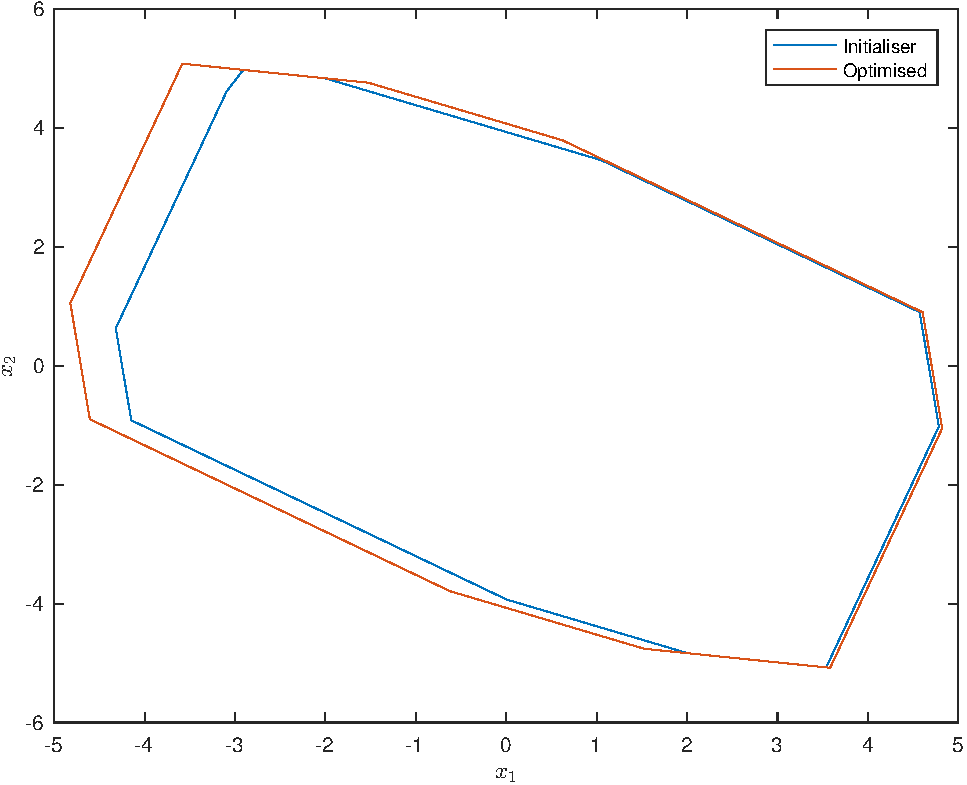
\includegraphics[width=.95\linewidth]{MRPIsetOptimised.pdf}
\caption{The guaranteed positively invariant set $X^\infty$ computed using~(\ref{seq:optimisation:MRPI:abstract}a-c) 
%of the system~\eqref{eq:example:system:MRPI} 
in red, and in blue the robust positively invariant set for the disturbance set computed using the methods discussed in~\cite{Zhang2015} with 
%a confidence level of $0.999$.}
confidence $1-\beta$, $\beta = 0.001$.}
\label{fig:MRPI:optimised}
\vspace{4mm}\end{figure}


For the same system and constraints (\ref{eq:example:system:MRPI})-(\ref{eq:example:pconstriaint}) we approximate the guaranteed 3-step controllable set $\C_3(\T)$, where $\T=\{x:\norm{x}_\infty\leq 2\}$
%
by solving (\ref{seq:optimisation:n:step:set:abstract}a-c) for $C_1(\T)$, $C_2(\T)$, $C_3(\T)$.
%
Again the result illustrated in Figure~\ref{fig:n:step:controllable:set} is reproduced using different initial values although the Hessian at the maximiser has a non-trivial nullspace.
%

\begin{figure}
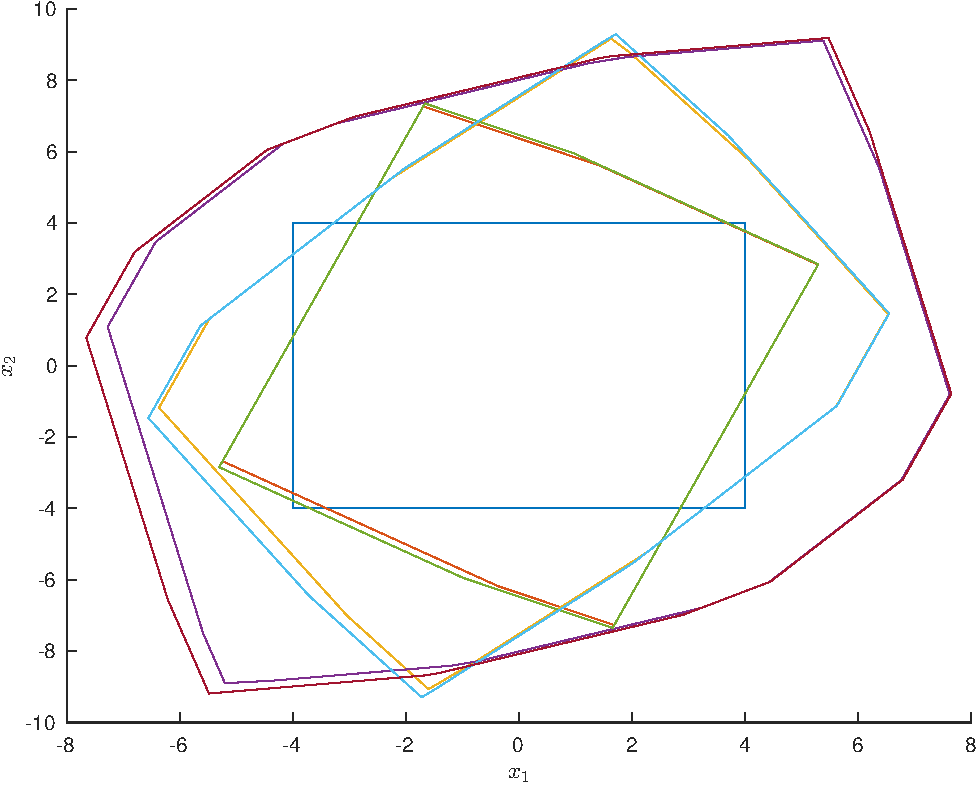
\includegraphics[width=.95\linewidth]{NStepSetOptimised.pdf}
\caption{Approximation of the guaranteed 3-step controllable set for a box $\T$ (in blue). Sets $C_1(\T)$, $C_2(\T)$ and $C_3(\T)$ computed by optimising $\V^\prime$ using  (\ref{seq:optimisation:n:step:set:abstract}a-c) are shown in solid lines. For comparison, the controllable sets obtained with~\eqref{eq:comparison:set} with 
confidence $1-\beta$, $\beta = 0.001$ are shown in dashed lines.}
\label{fig:n:step:controllable:set}
\vspace{4mm}\end{figure}



\section{Conclusions and future work}\label{sec:conclusion}
%
%
In this paper we present methods for approximating the positively invariant set and the $n$-step controllable set of a chance constrained stochastic system.
%
The approach we present is based on a simple restriction of the set $\V^\prime$ to be a parallelotope; this yields remarkable results in simulations and avoids the introduction of non-convex constraints in the optimisation problems (\ref{seq:optimisation:MRPI:abstract}a-c) and \mbox{(\ref{seq:optimisation:n:step:set:abstract}a-c)}.
 %

Although the presented scheme scales well to higher dimensions, the complexity of positively invariant sets and $n$-step controllable sets does not in general, and this could lead to computational intractability in the objective functions (\ref{seq:optimisation:MRPI:abstract}a) and (\ref{seq:optimisation:n:step:set:abstract}a) when the state dimension $d$ is large.
%

The underlying probability distribution was assumed to be uniform for ease of presentation, a similar method may be applied to more general distributions as long as they allow the probability measure of a parallelotope to be analytically determined.
%
Future work will remove this restriction by approximating non-uniform probability distributions as discrete distributions defined by collections of spatially distributed point masses.
%
This would necessarily introduce a degree of uncertainty in the probability measure of $\V^\prime$. However the uncertainty would be subject to deterministic bounds (rather than the statistical bounds provided by sample based approaches), which would allow for guarantees of constraint satisfaction. 



%\bibliographystyle{alpha}
\bibliography{MyBibliography}
\end{document}